\chapter{Herramientas}
\label{chap:herramientas}
En este capítulo se van a desarrollar las herramientas utilizadas en el desarrollo de este proyecto. Algunas se han elegido por facilidad su de uso y otras por necesidad del entorno desarrollado.

% JAVASCRIPT %
\section{JavaScript}
\label{sec:js}
\textit{JavaScript} es un lenguaje interpretado de alto nivel el cual se encuentra bajo el estándar \textit{ECMAScript}\footnote{Especificación de lenguaje de programación el cual define tipos dinámicos y soporta características de programación orientada a objetos.} y está basado en otros lenguajes de programación como Java o C.

En su principio, fue concebido como lenguaje para el lado cliente implementado en un navegador web permitiendo mejorar la interfaz de usuario y realizar páginas web dinámicas.
Actualmente, JavaScript se ha ido integrado en el lado servidor y es por ello que es el lenguaje más utilizado para desarrollo web y todos los navegadores interpretan el código integrado en las páginas web.
\subsection{Características}
Las siguientes características tienen en común que todas se ajustan al estándar de ECMAScript:
\begin{itemize}
    \item Es un lenguaje estructurado, tiene gran similitud con \textit{C} y comparte gran parte de su estructura (bucles, condicionales, sentencias...) a excepción del alcance de sus variables. En \textit{C} su ámbito es el bloque en el que fue definida y, en su origen, \textit{JavaScript} solo alcanzaba la función en la que es declarada. Es en ECMAScript 2015 cuando se añade la palabra clave \textit{let}, que incorpora compatibilidad con \textit{block scoping}.
    \item Tipado débil, por el cual el tipo de datos está asociado al valor, no a la variable. Esto significa que una variable puede ser \textit{number} o \textit{string} en distintos momentos de ejecución.
    \item Formado en su totalidad por objetos, en los cuales los nombres de las propiedades de los objetos son claves de tipo cadena siendo \textit{objeto.a = 1} y \textit{objeto['a'] = 1} equivalentes.
    \item función \textit{eval}, la cual evalúa un código en \textit{JavaScript} representado como una cadena de caracteres.


\end{itemize}
% A-FRAME %
\section{A-Frame}
\label{sec:aframe}
A-Frame es un framework de código abierto destinado a crear experiencias de realidad virtual a partir de \textit{HTML} de forma que sea sencillo de leer y comprender. De esta manera es accesible para crear una gran comunidad.



Además tiene compatibilidad con \textit{Vive}, \textit{Rift}, \textit{Windows Mixed Reality}, \textit{Daydream}, \textit{GearVR} y \textit{CardBoard} así como soporte para todos los controladores respectivos. También ofrece soporte para ordenadores de escritorio y para la mayoría de teléfonos inteligentes.

\subsection{HTML y primitivas}
\textit{A-Frame }se basa en \textit{HTML} y el \textit{DOM} usando un \textit{polyfill}\footnote{Fragmento de código en \textit{JavaScript} utilizado para proporcionar una funcionalidad moderna en navegadores antiguos.} para elementos personalizados. \textit{HTML} es un componente básico para Web y como tal, tiene una gran accesibilidad como lenguaje. Para crear una escena de realidad virtual con \textit{A-Frame} no se requiere ninguna instalación y simplemente con la creación del \textit{HTML} se puede abrir en el navegador. La mayoría de herramientas existentes(como \textit{React}, \textit{Vue.js}, \textit{d3.js} y \textit{jQuery}) funcionan en este framework.

\textit{HTML} y \textit{DOM} son solo la capa más externa del framework, debajo se encuentra el componente \textit{three.js} en el que está basado \textit{A-Frame} gracias al cual un componente puede ser utilizado en distintas entidades.

A-Frame proporciona elementos como \textit{$<a-box>$} o \textit{$<a-sky>$} llamados primitivas. Podemos crear un escenario a través de primitivas como el mostrado en la figura \ref{fig:scene1} con el código mostrado a continuación:


\begin{lstlisting}[caption=Código escenario primitivas]
<!DOCTYPE html>
<html>
  <head>
    <meta charset="utf-8">
    <title>Escenario primitivas</title>
    <script src="https://aframe.io/releases/0.9.2/aframe.min.js"></script>
  </head>
  <body>
    <a-scene background="color: #FAFAFA">
      <a-box position="-1 0.5 -3" rotation="0 45 0" color="#4CC3D9" shadow></a-box>
      <a-sphere position="0 1.25 -5" radius="1.25" color="#ff0000" shadow></a-sphere>
      <a-cylinder position="1 0.75 -3" radius="0.5" height="1.5" color="#FFC65D" shadow></a-cylinder>
      <a-plane position="0 0 -4" rotation="-90 0 0" width="4" height="4" color=" #1cde83" shadow></a-plane>
      <a-sky color="#e7e1e0"></a-sky>
    </a-scene>
  </body>
</html>
\end{lstlisting}


\begin{figure}[htb]
\centering
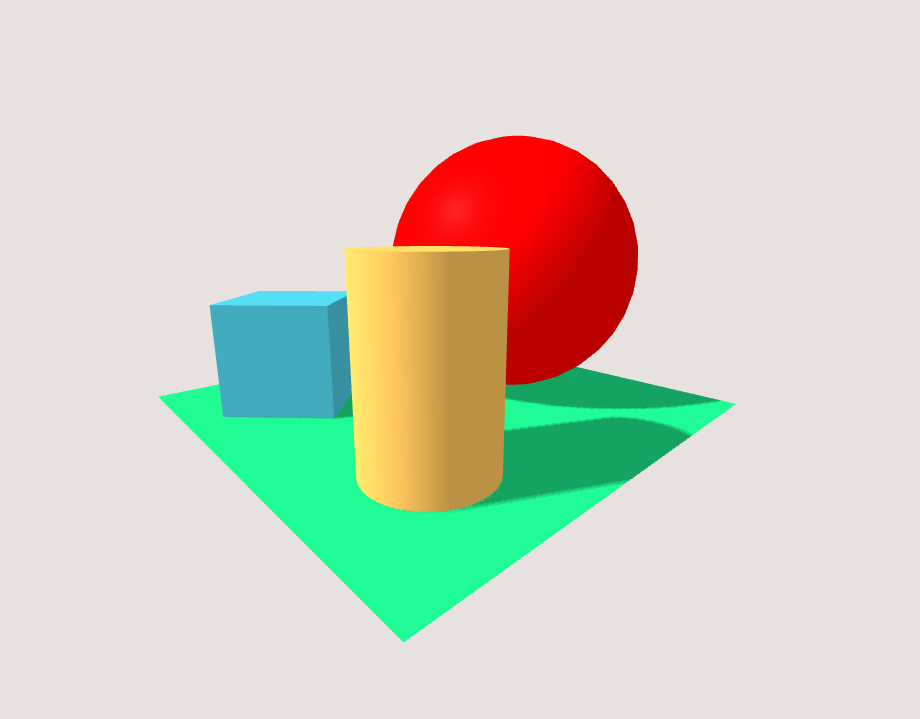
\includegraphics[width=0.8\textwidth]{img/scene1.png}
\caption{Escenario a-frame} \label{fig:scene1}
\end{figure}


% BLOCKLY %
\section{Blockly}
\label{sec:blockly}

% BLENDER %
\section{Blender}
\label{sec:blender}
\subsection{Modelos 3D}

% GESTORES DE PAQUETES %
\section{Gestores de paquetes}
\label{sec:gest}
\subsection{NPM}
\subsection{WebPack}

% WEBSIM %

\section{WebSim}
\label{sec:websim}
\begin{table}[h!]
  \begin{center}
    \caption{Métodos (HAL API) de los motores del robot.}
    \vspace{0.5cm}
    \label{tab:tabla-motores}
    \begin{tabular}{|c|c|}
    \hline
      \textbf{Método} & \textbf{Descripción}\\
      \hline
.setV(velLineal) & \begin{tabular}[c]{@{}c@{}}Mueve hacia delante o atrás el robot.\\\end{tabular} \\ \hline
.setW(velAngular) & \begin{tabular}[c]{@{}c@{}}Hace girar al robot.\\\end{tabular} \\ \hline
.move(velLineal, velAngular) & \begin{tabular}[c]{@{}c@{}}Mueve el robot hacia delante/atrás y gira al mismo tiempo.\\ \end{tabular} \\ \hline
.getV() & \begin{tabular}[c]{@{}c@{}}Obtener la velocidad lineal configurada en el robot.\\ \end{tabular} \\ \hline
.getW() & \begin{tabular}[c]{@{}c@{}}Obtener la velocidad angular configurada en el robot.\\ \end{tabular} \\ \hline
.getL() & \begin{tabular}[c]{@{}c@{}}Obtener la velocidad de elevación configurada en el robot.\\ \end{tabular} \\ \hline
    \end{tabular}
  \end{center}
\end{table}
